\section{Introduction}
\frame{\tableofcontents[currentsection]}


\begin{frame}
    % why partial optimality (not heuristic, approximation but no info about optimality)
    \frametitle{Problem Statement (1)}
    \onslide<1->{
        Finite sample set $\fSet$, 
        cost function $\cost \colon \binom{\fSet}{3} \to \real$.\\
        Instance of the \textbf{Cubic Clique Partition Problem}:\\
        \[
        \min\limits_{\labels \colon \binom{\fSet}{2} \to \bSet}
        \sum\limits_{abc \in \binom{\fSet}{3}}
        \cost_{abc}\labels_{ab}\labels_{bc}\labels_{ac} 
        \]
        subject to 
        $\labels_{ab} + \labels_{bc} - 1 \leq \labels_{ac}$
        for all distinct $a,b,c \in \fSet$.\\    
    }
    \vspace{25px}
    \onslide<2->{
        Find a \textbf{partially optimal solution}, i.e.
        fix some labels $\labels_{ab}$
        for distinct $a,b \in \fSet$
        \[
        \begin{cases}
            \labels_{ab}=1 & \text{join } a,b\\
            \labels_{ab}=0 & \text{cut } a,b\\
            \labels_{ab}=\text{?} & \text{unknown}
        \end{cases}
        \]
        in such way that there still exists
        an optimal solution. 
    }
\end{frame}

\begin{frame}
    \frametitle{Problem Statement (2)}
    \textbf{Subspace Instances} of the Cubic Clique Partition Problem
    \vspace{5px}
    \onslide<1->{
        Samples $\fSet$: points $\fSet \subset \real^3$\\
    }
    \onslide<2->{
        Point generation: 3 distinct planes containing the origin, noise $\noise$\\
    }
    \onslide<3->{
        Optimal labeling $\labels^*$: original planes\\
    }
    \onslide<4->{
        Cost function $\cost$? (no concrete plane information given)
    }
    \begin{figure}[h]
    \centering
        \onslide<1->{
            \begin{subfigure}{0.4\textwidth}
                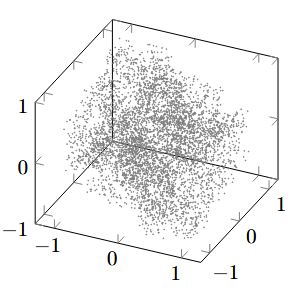
\includegraphics[width=\textwidth]{gray-points}
                \caption{Samples $\fSet$}
            \end{subfigure}
        }
        \hfill
        \onslide<2->{
            \begin{subfigure}[b]{0.4\textwidth}
                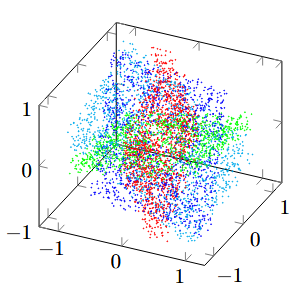
\includegraphics[width=\textwidth]{colored-points}
                \caption{Optimal labeling $\labels^*$}
            \end{subfigure}
        }
        \hspace{0.1\textwidth}
    \end{figure}
\end{frame}


\begin{frame}
    \frametitle{Research Goals and Contributions}
    \onslide<1->{
    \textbf{Related Work:}\\
    TODO: 2 + 1 \\
    }
    \vspace{5px}
    \onslide<2->{
    \textbf{Tasks and Solutions:}
    \begin{enumerate}
        \onslide<2->{
        \item Read TODO, implement the partial optimality algorithm\\
        $\to$ implementation in C++ (with some adjustments)  
        }
        \onslide<3->{
        \item Construct subspace instances of increasing difficulty\\
        $\to$ point generation, appropriate cost function $\cost$\\
        (significant noise tolerance) 
        } 
        \onslide<4->{
        \item Apply algorithm to the subspace instances,
        assess partial optimality, accuracy and computation time\\
        $\to$ experiments and evaluation 
        (prove the quality of $\cost$)
        }
    \end{enumerate}
    }
    % Paper (basiert sich auf 2 unten)
    % https://arxiv.org/abs/1812.01426
    % https://scholar.google.com/citations?view_op=view_citation&hl=de&user=qdVbsUYAAAAJ&citation_for_view=qdVbsUYAAAAJ:2osOgNQ5qMEC

    % \begin{tabularx}{\textwidth}{p{0.5\textwidth}|X}
    %     \textbf{Task} & \textbf{Solution}\\
    %     \hline 
    %     \onslide<1->{
    %     \vspace{-7px}
    %     read
    %     `Partial Optimality in Cubic Correlation Clustering'
    %     \cite{TODO};
    %     implement the algorithm for establishing partial optimality
    %     to the cubic clique partition problem;
    %     } &
    %     \onslide<2->{
    %     \vspace{-7px}
    %     my own implementation in C++ of the suggested
    %     algorithm with some adjustments
    %     \\
    %     \hline
    %     }
    %     \onslide<3->{
    %     \vspace{-7px}
    %     construct subspace instances
    %     of increasing difficulty
    %     by generating the sample points
    %     and by defining a
    %     \textbf{suitable cost function}
    %     for the point triples
    %     } &
    %     \onslide<4->{
    %     \vspace{-7px}
    %     point generation using the linear algebra methods;
    %     experimentally determined geometric
    %     cost function 
    %     with a significant noise tolerance;
    %     \\
    %     \hline
    %     }
    %     \onslide<5->{
    %     \vspace{-7px}
    %     apply the algorithm to the constructed subspace instances,
    %     assess partial optimality, accuracy with respect to
    %     truth, and computation time
    %     } &
    %     \onslide<6->{
    %     \vspace{-7px}
    %     systematic empirical assessment
    %     of the algorithm application to the problem subspace instances 
    %     with my cost function proving its quality
    %     }
    % \end{tabularx}
\end{frame}
